% THIS IS SIGPROC-SP.TEX - VERSION 3.1
% WORKS WITH V3.2SP OF ACM_PROC_ARTICLE-SP.CLS
% APRIL 2009
%
% It is an example file showing how to use the 'acm_proc_article-sp.cls' V3.2SP
% LaTeX2e document class file for Conference Proceedings submissions.
% ----------------------------------------------------------------------------------------------------------------
% This .tex file (and associated .cls V3.2SP) *DOES NOT* produce:
%       1) The Permission Statement
%       2) The Conference (location) Info information
%       3) The Copyright Line with ACM data
%       4) Page numbering
% ---------------------------------------------------------------------------------------------------------------
% It is an example which *does* use the .bib file (from which the .bbl file
% is produced).
% REMEMBER HOWEVER: After having produced the .bbl file,
% and prior to final submission,
% you need to 'insert'  your .bbl file into your source .tex file so as to provide
% ONE 'self-contained' source file.
%
% Questions regarding SIGS should be sent to
% Adrienne Griscti ---> griscti@acm.org
%
% Questions/suggestions regarding the guidelines, .tex and .cls files, etc. to
% Gerald Murray ---> murray@hq.acm.org
%
% For tracking purposes - this is V3.1SP - APRIL 2009

\documentclass{acm_proc_article-sp}

\usepackage{algorithm}
\usepackage{algorithmic}

\begin{document}

\title{Solving the grand challenge using an algorithmic an distributed approach}
%
% You need the command \numberofauthors to handle the 'placement
% and alignment' of the authors beneath the title.
%
% For aesthetic reasons, we recommend 'three authors at a time'
% i.e. three 'name/affiliation blocks' be placed beneath the title.
%
% NOTE: You are NOT restricted in how many 'rows' of
% "name/affiliations" may appear. We just ask that you restrict
% the number of 'columns' to three.
%
% Because of the available 'opening page real-estate'
% we ask you to refrain from putting more than six authors
% (two rows with three columns) beneath the article title.
% More than six makes the first-page appear very cluttered indeed.
%
% Use the \alignauthor commands to handle the names
% and affiliations for an 'aesthetic maximum' of six authors.
% Add names, affiliations, addresses for
% the seventh etc. author(s) as the argument for the
% \additionalauthors command.
% These 'additional authors' will be output/set for you
% without further effort on your part as the last section in
% the body of your article BEFORE References or any Appendices.

\numberofauthors{2} %  in this sample file, there are a *total*
% of EIGHT authors. SIX appear on the 'first-page' (for formatting
% reasons) and the remaining two appear in the \additionalauthors section.
%
\author{
% You can go ahead and credit any number of authors here,
% e.g. one 'row of three' or two rows (consisting of one row of three
% and a second row of one, two or three).
%
% The command \alignauthor (no curly braces needed) should
% precede each author name, affiliation/snail-mail address and
% e-mail address. Additionally, tag each line of
% affiliation/address with \affaddr, and tag the
% e-mail address with \email.
%
% 1st. author
\alignauthor
Amila Suriarachchi\\
       \affaddr{Colorado State University}\\
       \affaddr{Fort Collins}\\
       \affaddr{Colorado}\\
       \email{amilas@cs.colostate.edu}
% 2nd. author
\alignauthor
Shrideep Pallickara\\
       \affaddr{Colorado State University}\\
       \affaddr{Fort Collins}\\
       \affaddr{Colorado}\\
       \email{shrideep@cs.colostate.edu}
}
% There's nothing stopping you putting the seventh, eighth, etc.
% author on the opening page (as the 'third row') but we ask,
% for aesthetic reasons that you place these 'additional authors'
% in the \additional authors block, viz.
% Just remember to make sure that the TOTAL number of authors
% is the number that will appear on the first page PLUS the
% number that will appear in the \additionalauthors section.

\maketitle
\begin{abstract}
Processing complex queries on unbounded event streams in real time, is a challenge for many organizational data processing systems. These systems are expected to process data with minimal latency to generate real time events, and high through put to minimize the required hardware. In this regard DEBS Grand Challenge 2015 focus on evaluating two queries (frequent routes and  profitable cells) in real time with minimal latency and high throughput. These queries involve processing windows of thousands of records. Firstly, such processing demands efficient data structures and algorithms to minimize the processing over head. Secondly, system should partition data to process them in parallel to efficient use of hardware.

In this paper, we present a set of data structures which can be used to evaluate two queries with O(log(n)) time complexity and a data partition technique to process events in parallel. Then we evaluate our solution within signal node as well as in distributed setups. We could process frequent routes query with 173 million dataset within 5 minutes with less than 4 millisecond latency and profitable cells query with same data set within 11 minutes with less than 5 millisecond latency.
\end{abstract}

% A category with the (minimum) three required fields
%A category including the fourth, optional field follows...

\keywords{DEBS Grand Challenge, Distributed Event Processing, Time Complexity} % NOT required for Proceedings

\section{Introduction}
introduction

\section{Query Implementation}
In this section, we elaborate how we have implemented the query logic to achieve O(log(n)) time complexity. The 2015 Grand Challenge problem has two queries. First is to evaluate top ten most frequent routes within last 30 minutes and second is to evaluate top ten profitable areas within last 15 minutes. We can use a composite object to keep route details for each route and fare details to each cell to compare values among routes and cells. However, each time window can have thousands of route and cell details. Therefore an efficient data structure is required to add, remove, update and retrieve top ten values from a set of objects for a given time window efficiently. Further since each event is received with route and cell details, above mentioned operations should perform using route and cell details as the key. In order to support all these functions with O(log(n)) time complexity we developed a data structure called \textit{NodeList}. Following parts of this section describes how we have achieve this time complexity with \textit{NodeList} data structure and how we have implemented the queries using that data structure.

\subsection{NodeList data structure}

\begin{table}
\centering
\caption{Operations of \textit{NodeList} Data Structure}
\begin{tabular}{|l|l|} \hline
Operation Signature & Time Complexity \\ \hline \hline
add(key : Object, value : NodeValue) & O(log(n)) \\ \hline 
get(key : Object) : NodeValue & O(1) \\ \hline
remove(key : Object) : NodeValue & O(log(n)) \\ \hline
decrementPosition(key : Object) & O(log(n)) \\ \hline
incrementPosition(key : Object) & O(log(n)) \\ \hline
getTopValues() : List<NodeValue> & O(1) \\ \hline
\end{tabular}
\label{nodelist_api}
\end{table}

Table \ref{nodelist_api} shows the operations of this data structure. The \textit{NodeValue} is an interface to plug any user defined type as a value. For an example, the route query can use a \textit{RouteCount} object to keep route count while profitable cells query can use \textit{CellProfict} object to keep fare details. This interface contains a method called compare to define the order of the values. The \textit{NodeList} data structure provides the notion of a sorted values starting from position 0 (highest value) to its users. The \texttt{decrementPostion} operation moves the corresponding value towards position 0 until the correct position according to sorted order. Therefore this method should be called after increasing a value of an existing object. Similarly \texttt{incrementPosition} operation can be used to move a value to correct position after decreasing the value of an existing object. \texttt{GetTopValues} operation returns the top ten values of the list. Query algorithm sections further elaborate usage of these methods.

One way of implementing this data structure is to use a heap. Heap supports adding and extracting maximum value operations in O(log(n)) time. However since this application requires top 10 values, we need to retrieve maximum value ten times and insert them back. On the other hand if we use a doubly linked list to keep values, it will take O(n) time for  \texttt{decrementPostion} and \texttt{incrementPosition} operations. Therefore we can use a doubly linked list to keep first 10 values (this makes time complexity for all operations with this data structure O(1)) and a heap to keep other values to avoid above problems.  A \textit{Map} which points to values can be used to retrieve values using a key.

\textit{NodeList} data structure uses two data structures called \textit{OrderedList} to keep first 10 values and \textit{DynamicHeap} to keep other values. In this way it has to change only the last value of \textit{OrderedList} and maximum value of \textit{DynamicHeap} as required. Following sections describes how these data structures have been implemented with their operations.

\subsection{OrderedList data structure}

\begin{table}
\centering
\caption{Operations of \textit{OrderedList} Data Structure}
\begin{tabular}{|l|l|} \hline
Operation Signature & Time Complexity \\ \hline \hline
add(key : Object, value : NodeValue) & O(n) \\ \hline
containsKey(key : Object) : boolean & O(1) \\ \hline
get(key : Object) : NodeValue & O(1) \\ \hline
incrementPosition(key : Object) & O(n) \\ \hline
decrementPosition(key : Object) & O(n) \\ \hline
remove(key : Object) : NodeValue & O(1) \\ \hline
getLastPosition() : int & O(1) \\ \hline
getLastKey() : Object & O(1) \\ \hline
\end{tabular}
\label{orderedlist_api}
\end{table}

Table \ref{orderedlist_api} shows the operations of the \textit{OrderedList} data structure. First six methods has the same meanings as the \textit{NodeList} data structure and last two can be used to get the size of the list and the value of the last object. We internally keep a counter and a pointer to tail to support these operations in O(1) time. Figure \ref{orderedlist_impl} shows the implementation details. The \textit{Map} structure (an \textit{java.util.HashMap}) is used to retrieve object pointers with O(1) expected time. Each node of the doubly linked list points to previous and next nodes while storing the \textit{NodeValue}.


\begin{figure}[!t]
        \centering
        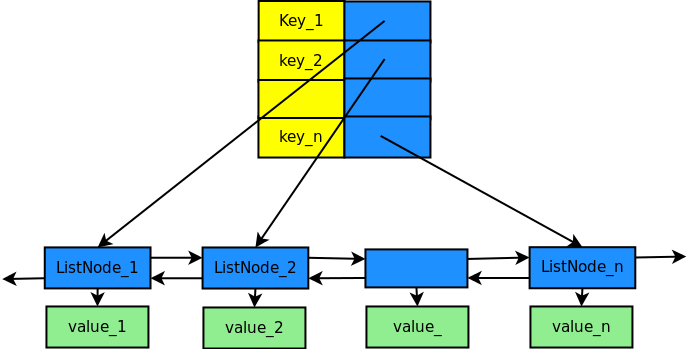
\includegraphics[width=3.0in]{orderedlist.png}
        \caption{\textit{OrderedList} data structure implementation}
        \label{orderedlist_impl}
\end{figure}

\subsection{DynamicHeap data structure}

\begin{table}
\centering
\caption{Operations of \textit{DynamicHeap} Data Structure}
\begin{tabular}{|l|l|} \hline
Operation Signature & Time Complexity \\ \hline \hline
add(key : Object, value : NodeValue) & O(log(n)) \\ \hline
remove(key : Object) : NodeValue & O(log(n)) \\ \hline
containsKey(key : Object) : boolean & O(1) \\ \hline
get(key : Object) : NodeValue & O(1) \\ \hline
moveUp(key : Object) & O(log(n)) \\ \hline
moveDown(key : Object) & O(log(n)) \\ \hline
getMaxkey() : Object & O(1) \\ \hline
extractMax() : NodeValue & O(log(n)) \\ \hline
\end{tabular}
\label{dynamicheap_api}
\end{table}

Table \ref{dynamicheap_api} shows the operations of the \textit{DynamicHeap} data structure. \texttt{MoveUp} and \texttt{moveDown} operations are used to move an element up in the heap if the value increased, or move down in the heap if the value decreased. Figure \ref{dynamicheap_impl} shows the implementation details. Conventional heaps only support \texttt{add} and \texttt{extractMax} operations since heap operations requires to know the element position in heap. When adding an element, we add it to last position and move that up and extracting maximum element start at array position 0. In order to support \texttt{moveUp}, \texttt{moveDown} and \texttt{remove} operations, we keep the array index with the object itself. This allows us to retrieve array index in O(1) time and move the element O(log(n)) time.


\begin{figure}[!t]
        \centering
        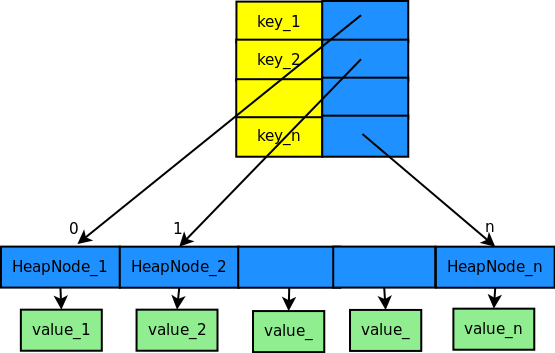
\includegraphics[width=3.0in]{DinamicHeap.png}
        \caption{\textit{DynamicHeap} data structure implementation}
        \label{dynamicheap_impl}
\end{figure}

\subsection{Frequent Route Query}

Frequent route query requires to find the top frequent routes within last 30 minutes. Algorithm \ref{frequent_route_algorithm} shows the algorithm to process this query using the \textit{NodeList} data structure and a queue to keep the events for the time window.  Since queue operations are supported in O(1) time, query evaluation happens in O(log(n)) time. Algorithm \ref{frequent_route_algorithm} shows the basic algorithm to process an event. This algorithm assumes there is a global \textit{NodeList} object and route counts stored in an Object called \textit{RouteCount}. 

\begin{algorithm}
\caption{Algorithm to generate top 10 frequent route change events}
\label{frequent_route_algorithm}
\begin{algorithmic}
\small 
\STATE beforeTopTen $\leftarrow$ nodeList.getTopValues() 
\STATE window.add(event) 
\IF{ nodeList.containsKey(event.route) }
	\STATE routCount $\leftarrow$ nodeList.get(event.route) 
	\STATE routCount.count++ 
	\STATE nodeList.decrementPosition(event.route) 
\ELSE
	\STATE nodeList.add(event.route, new RouteCount(1)) 
\ENDIF

\WHILE{ there exists expired events }
	\STATE  expEvent $\leftarrow$ window.poll() 
	\STATE  routCount $\leftarrow$ nodeList.get(expEvent.route)
	\STATE  routCount.count-- 
	\IF{ routCount.count is 0 }
		\STATE nodelist.remove(expEvent.route)
	\ELSE
		\STATE nodeList.incrementPosition(expEvent.route) 
	\ENDIF
\ENDWHILE

\STATE nowTopTen $\leftarrow$ nodeList.getTopValues() 

\IF{ preTopTen not equals nowTopTen }
	\STATE create new event with top ten route details 
\ENDIF

\end{algorithmic}
\end{algorithm}

Processing an event can cause add, remove or update values of the existing time window objects. Therefore query processing mainly involves with performing above operations to the underlying \textit{NodeList} data structure and compare before and after top ten routes. As shown in Algorithm \ref{frequent_route_algorithm}, when an event arrives, first it puts the event to time window to keep track for last 30 minutes. Then it adds new route value or updates the existing value and moves its position. Similarly, for expired events either it removes the values or reduces the count for existing values. Finally, two lists are compared to decide whether to generate an event or not. Here we have given a rough outline of the algorithm. Real implementation considers other factors such as sequence number to order events.

\subsection{Profitable Cells Query}

We have implemented profitable cells query in a similar manner to the frequent route query using  time windows. Complexity of the query raised following issues and we have solved them as given bellow.
\begin{enumerate}
	\item The profitability is calculated using the median profit and the number of empty taxis. In order to calculate median with O(log(n)) time complexity, we use two heaps (\textit{java.util.PriorityQueue}) . One is used to keep the values lesser than the median value (max heap) and other is to keep higher values (min heap). However the \texttt{delete} operation of \textit{java.util.PriorityQueue} takes O(n) time, since it traverse along the array to find the index of the object. We tried with our \textit{DynamicHeap} implementation to fix this. But that did not improved the performance. Firstly, these heap sizes does not grow over the value of 145 and there are same values repeating in the list increasing the probability of find a value without traversing the whole list. Secondly, our implementation create more objects compared to just keeping double values though the time complexity is O(log(n)). 
	\item In order to keep tract of empty taxis, we need to process both pickup cell and dropoff cell details for each message. One way of doing this is to send all events for same process instance and process both details with one event. However this avoid the possibility of partitioning data across different processes. We generate two events, one for pickup data and one for dropoff data to make the process parallel. 
	\item In order to handle expiration of dropoff events, we keep track of the taxi ids currently available in a particular cell. If a pickup event occurs before dropoff event expiration, then we remove that taxi id from that cell and reduce the empty taxi count. In such a case dropoff event expiration does not cause a reduction of taxi count.
\end{enumerate}

Algorithm \ref{pickup_algorithm} shows the logic to process pickup data. When a taxi gets a pickup, the taxi fare is added to that cell. We use \textit{ProfitCellNode} to keep the fare and empty taxi details to calculate the profitability. Then if its' taxi dropoff event has not been occurred (i.e this taxi has come to this location less than 30 minutes ago) it removes the taxi from that location. When the event get expired, it removes the fare from the \textit{ProfitCellNode}. 

\begin{algorithm}
\caption{Algorithm to process pickup data}
\label{pickup_algorithm}
\begin{algorithmic}
\small
\STATE beforeTopTen $ \leftarrow $ nodeList.getTopValues()
\STATE paymentWindow.add(event)
\IF {nodeList.containsKey(event.pickUpCell)}
	\STATE profitCellNode $ \leftarrow $ nodeList.get(event.pickUpCell)
	\STATE profitCellNode.addFare(event.fare)
	\IF {profitCellNode.containsTaxi(event.medalliion)}
		\STATE profitCellNode.emptyTaxi--
		\STATE profitCellNode.removeTaxi(event.medallion)
	\ENDIF
	\IF {profitablity has increased}
		\STATE nodeList.decrementPosition(event.pickUpCell)
	\ELSE
		\STATE nodeList.incrementPosition(event.pickUpCell)	
	\ENDIF
\ELSE
	\STATE nodeList.add(event.pickUpCell, new ProfitCellNode(event.fare))
\ENDIF
\WHILE {there exits expired events}
	\STATE expiredEvent $ \leftarrow $ paymentWindow.poll()
	\STATE profitCellNode $ \leftarrow $ nodeList.get(expiredEvent.pickUpCell)
	\STATE profitCellNode.removeFare(expiredEvent.fare)
	
	\IF {profitCellNode is empty}
		\STATE nodeList.remove(expiredEvent.pickUpCell)
	\ELSIF {profitablity increased}
		\STATE nodeList.decrementPosition(event.pickUpCell)
	\ELSE
		\STATE nodeList.incrementPosition(event.pickUpCell)
	\ENDIF
\ENDWHILE
\STATE nowTopTen $ \leftarrow $ nodeList.getTopValues()
\IF {beforeTopTen not equals to nowTopTen}
	\STATE emit a top ten change event
\ENDIF		 

\end{algorithmic}
\end{algorithm}

Algorithm \ref{dropoff_algorithm} shows the logic to process dropoff data. When a taxi trip ended in a location, number of empty taxis of that location has to be increased. If the taxi does not get a pickup within 30 mintes, then that taxi has to be removed from that location.

\begin{algorithm}
\caption{Algorithm to process dropoff data}
\label{dropoff_algorithm}
\begin{algorithmic}
\small
\STATE beforeTopTen $ \leftarrow $ nodeList.getTopValues()
\STATE dropWindow.add(event)
\IF {nodeList.containsKey(event.dropOffCell)}
	\STATE profitCellNode $ \leftarrow $ nodeList.get(event.dropOffCell)
	\STATE profitCellNode.addTaxi(event.medallion)
	\STATE profitCellNode.emptyTaxi++
	\STATE nodeList.incrementPosition(event.dropOffCell)	

\ELSE
	\STATE nodeList.add(event.dropOffCell, new ProfitCellNode(event.medallion))
\ENDIF
\WHILE {there are expired events}
	\STATE expiredEvent $ \leftarrow $ dropWindow.poll()
	\STATE profitCellNode $ \leftarrow $ nodeList.get(expiredEvent.dropOffCell)
	\IF {profitCellNode.containsTaxi(expiredEvent.medallion)}
		\STATE profitCellNode.emptyTaxi--
		\STATE profitCellNode.removeTaxi(expiredEvent.medallion)
		
		\IF {profitCellNode is empty}
			\STATE nodeList.remove(event.dropoffCell)
		\ELSE 
			\STATE nodeList.decrementPosition(event.dropOffCell) 
		\ENDIF
	\ENDIF
\ENDWHILE

\end{algorithmic}
\end{algorithm}






\section{Query evaluation}

In this section, we explain how to evaluate queries with the given data set. For this query evaluation we can use a distributed event stream processing system with the process graph as shown in Figure \ref{twonode_graph} for both queries.

\begin{figure}[!t]
        \centering
        \includegraphics[width=2.0in]{twonode_graph.png}
        \caption{Two node process graph to evaluate queries}
        \label{twonode_graph}
\end{figure}

\textit{EventEmitter} reads the data file and generates events with a sequence number. This sequence number is used to order \textit{QueryEvaluator} results. For real implementation, each query has its own \textit{EventEmitter} that reads each line of the data file and generates an event with the relevant information. \textit{QueryEvaluator} evaluates the query against the received event and generates top ten value changed event.  In general we can evaluate queries sequentially and in parallel. In a sequential execution, all events goes to one \textit{QueryEvaluator} instance and in a parallel execution, the event stream is partitioned using the key field and evaluate simultaneously with different \textit{QueryEvaluator} instances.

\subsection{Sequential evaluation}

We can sequentially execute events either in a single Java Virtual Machine (JVM) or in different JVMs (either in one machine or different machines) using TCP sockets to communicate among process instances. Figure \ref{sequential} shows possible executions. 

\begin{figure}[!t]
        \centering
        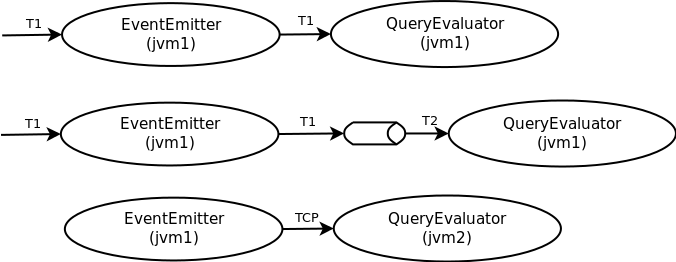
\includegraphics[width=3.0in]{sequential.png}
        \caption{Different types of sequential execution}
        \label{sequential}
\end{figure}

First both processors can be executed in same JVM with same thread. In that case, both processes execute sequentially. We can make two processes parallel by executing them with two threads and communicate using a queue in same JVM or communicate using a TCP connection for different JVMs. In all these cases \textit{QueryEvaluator} processes messages sequentially and becomes the bottleneck. Next we show how to parallel \textit{QueryEvaluator} process. 

\subsection{Parallel evaluation}
The general way to parallelize event processing, is to partition the events according to a key and run multiple instances to process data. Therefore in this section, we explain how to parallelize the query evaluation process taking frequent route query into consideration. Same concepts can be applied to profitable cell evaluation as well.

For frequent route query, route events can be partitioned using the hash code of the route object and process different route sets in different \textit{QueryEvaluators}. In such a setup, each \textit{QueryEvaluator} generates an event when the top ten routes get changed for its route set. Since this is not the desired result, we can add another process to aggregate these top result events and generate global route change events. Figure \ref{parallel} shows, possible parallel evaluation techniques with the new process. Multiple \textit{QueryEvaluator} instances can be executed in a single JVM using multiple threads or in a distributed setup with many JVMs using TCP to communicate. 

\begin{figure}[!t]
        \centering
        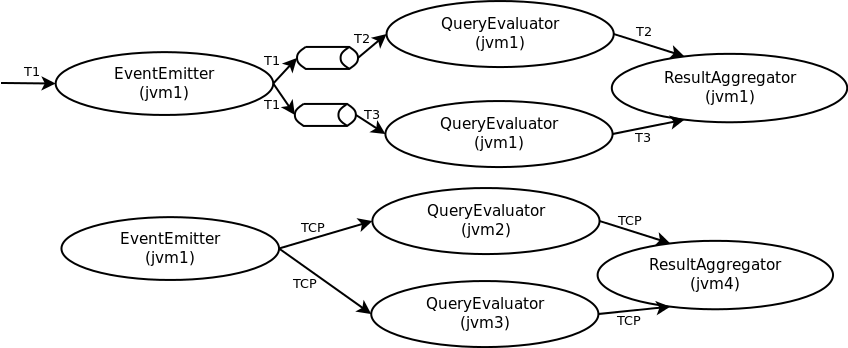
\includegraphics[width=3.0in]{parallel.png}
        \caption{Different types of parallel execution}
        \label{parallel}
\end{figure}

\textit{ResultAggregator} keeps a set of route counts received by \textit{QueryEvaluators}. Upon receiving a new event, it can update the existing route count values and check whether the global top ten route counts have changed. If there is a change, it can generate a top ten route changed event. This logic has the following issues and can be fixed as given bellow.

\begin{enumerate}
	\item \textbf{Expired values} : Route count of a particular route can be reduced due to expiration of some events. For an example, lets assume route count for route R1 is 10 and R1 is included in a top ten route event generated by a \textit{QueryEvaluator}. Then lets assume when the next event is generated, the route count for R1 has been reduced to 7 (due to expiration events) and hence R1 is not included in the next top ten route event. However since R1 value still is in the \textit{ResultAggregator} that may produce an event with this value. To avoid this problem, we send the removed route set details with the top ten route event generated by the \textit{QueryEvaluator}. In that case \textit{ResultAggregator} can first remove those routes.
	\item \textbf{Out of order events} : \textit{ResultAggregator} may receive events in a different order than those are produced at the \textit{EventEmitter}. This out of order events may change the final output of the \textit{ResultAggregator}. We order messages at the \textit{ResultAggregator} to avoid this problem. In order to order messages, we keep a message queue for each \textit{QueryEvaluator} and sent the message with least sequence number to \textit{ResultAggregator},  if a message is present in all queues. 
	\item \textbf{Intermediate top ten route events} : A route event increases the route count for that events' route. Further that can generate some expiration events which may reduce the route count for other routes. The top ten frequent routes can be changed due to these expiration events as well. Lets say in one \textit{QuerayEvaluator} case, a particular event causes two routes R1 and R2 to change and generates a top ten route change event. In the distributed setup these two routes can be in two \textit{QueryEvaluators} and that can cause two top ten route change events. These two events may result in two top ten route change events at \textit{ResultAggregator} as well instead of one. Further we observed only around 5\% of such events are generated, and system goes to the one \textit{QueryEveluator} result after all such event are being executed. Solution for such a problem may depend on the nature in which a real application, uses these results in decision making process. Therefore we could not provide any fix for this problem.
\end{enumerate}

Algorithm \ref{aggregate_algorithm} shows the algorithm for ResultAggregator with above fixes. First it removes the expired keys. Then it updates the existing values or adds new values and moves the position in the list accordingly. Finally it generates an event if there is a change to the top list.


\begin{algorithm}
\caption{Algorithm to aggregate top ten results from QueryEvaluators and generate global events}
\label{aggregate_algorithm}
\begin{algorithmic}

\STATE preTopTen $\leftarrow$ nodeList.getTopValues()
\FORALL {key in event.removedKeys}
	\STATE nodeList.remove(key)
\ENDFOR

\FORALL {nodeValue in event.newValuesList}
	\IF {nodeList.containsKey(nodeValue.key)}
		\STATE existingValue $\leftarrow$ nodeList.get(nodeValue.key)
		\IF { existing value is lesser than current }
			\STATE update the existing value
			\STATE nodeList.decrementPosition(nodeValue.key)
		\ELSE
			\STATE update the existing value
			\STATE nodeList.incrementPosition(nodeValue.key)
		\ENDIF
	\ELSE
		\STATE nodeList.add(nodeValue.key, nodeValue)
	\ENDIF
\ENDFOR

\STATE nowTopTen $\leftarrow$ nodeList.getTopValues()
\IF { preTopTen not equals nowTopTen }
	\STATE emit new event
\ENDIF
\end{algorithmic}
\end{algorithm}

\section{Experiments}
We conducted several experiments to study the scalability of our solution. Firstly we study the throughput and mean message latency variation with the number of \textit{QueryEvaluators} for both single JVM and distributed setups to find the scalability of the parallel evaluation. We measured the end to end latency. At the \textit{EventEmitter}, we set the time stamp for all events once the record is read. At the \textit{QueryEvaluator} we copy the original time stamp, if that event causes a top ten value change event. Total delay calculated at the \textit{ResultAggregator} just before writing the event. In an ideal system, we should observe linear throughput increment with a constant message latency. However there are some exceptions and we have provided our explanations on them. Finally we studied the throughput variation with the window size to study the suitability of our solution for higher window sizes. All these experiments were performed on a LAN with a network bandwidth of 1Gbps and all machines were Intel(R) Xeon(R) 2.4GHz, 4 core duo machines with 16 GB of memory. 

\subsection{Frequent routes query}

\begin{figure}[!t]
        \centering
        \includegraphics[width=3.0in]{routegraph.png}
        \caption{Process graph to evaluate top ten frequent routes.}
        \label{routegraph}
\end{figure}

Figure \ref{routegraph} shows the process graph used to process frequent route queries. \textit{RouteEventEmitter} reads the data file and emits events with a sequence number. \textit{RouteEmitter} contains a set of threads (equals to the number of \textit{RouteProcessors}) to emit events more efficiently. When processing each line first it reads the data line and creates a \textit{Route} object using longitude and latitude coordinates of pickup and dropoff locations. Then it distributes the events among the \textit{RouteProcessors} using the hash value of the \textit{Route} object. \textit{TopRouteProcessor} aggregates the results and saves them to a file.

We deployed this process graph to a distributed stream processing system we have developed, and  measured the throughput and the mean message latency varying the number of \textit{RouteProcessors} with the data set given (173 million records). In the local set up, we use a new thread to execute a new instance and in the distributed setup we add a new node to execute the new instance.

\begin{figure}[!t]
        \centering
        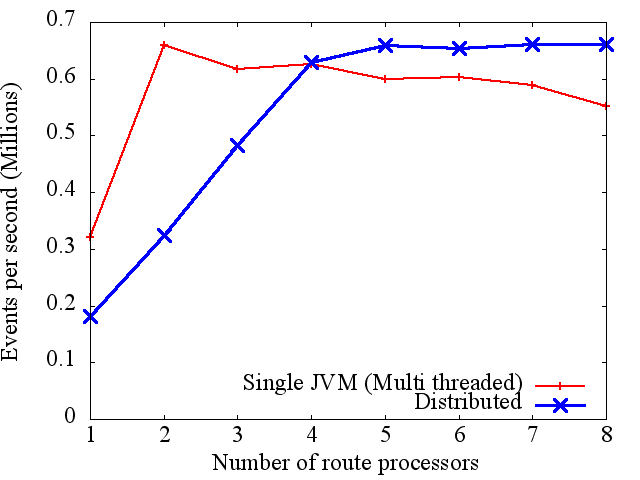
\includegraphics[width=3.0in]{throughput_route.png}
        \caption{Throughput variation with the number of \textit{RouteProcessor} instances.}
        \label{throughput_route}
\end{figure}

Figure \ref{throughput_route} shows the throughput variation. For single JVM setup throughput increases from one instance to two instances. This is due to higher parallelism system achieves with two threads. After that throughput slightly decreases due to higher context switching with many threads. Similarly for distributed setup initially throughput increases with the number of   \textit{RouteProcessors} and achieves a steady limit. We observe two reasons for this non scalability after initial stages. Firstly, \textit{RouteProcessor} is not a computing intensive process. Secondly, there is only one \textit{RouteEventEmitter} and the speed at which it can read and send messages becomes the bottleneck. Initial throughput for distributed setup is less, due to message serialization, message deserialization and TCP overheads. 

\begin{figure}[!t]
        \centering
        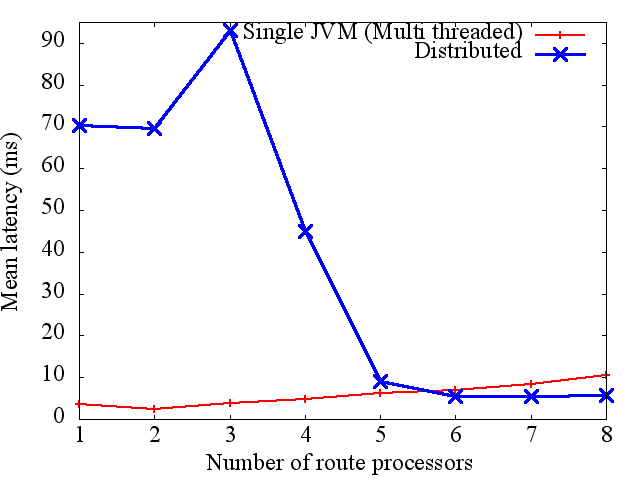
\includegraphics[width=3.0in]{latency_route.png}
        \caption{Mean latency variation with the number of \textit{RouteProcessor} instances.}
        \label{latency_route}
\end{figure}

Figure \ref{latency_route} shows the latency variation. For single JVM setup latency get reduced at 2 and slightly increases after that due to context switching overhead with higher number of threads. For distributed setup there is an high initial latency due to communication overheads. After that it comes to a constant value. 

\subsection{Profitable cells query}

\begin{figure}[!t]
        \centering
        \includegraphics[width=3.0in]{profitgraph.png}
        \caption{Process graph to evaluate top ten profitable cells.}
        \label{profictgraph}
\end{figure}

Figure \ref{profictgraph} shows the process graph for profitable cells query. \textit{ProfitEventEmitter} reads the data file and calculates the pickup cell and dropoff cell details using longitude and latitude coordinates. Then it creates two events one for dropoff part and other to pickup part, with different sequence numbers and distributes the events among \textit{ProfitCalculators} using the hash value of the cell. In this way cells are partitioned into different \textit{ProfitCalculator} instances and each instance gets all the events relevant to its' cell set. We use a set of threads (equals to the number of Profict Calculators) to emit data as in the previous query. Finally \textit{TopProfitProcessor} aggregates events and writes to a file. 

Similar to earlier experiment,  we deployed this process graph to our system and measured the throughput and the average message latency increasing the number of  \textit{ProfitCalculaor} instances for both single JVM setup and distributed setup to examine the scalability of our solution.

\begin{figure}[!t]
        \centering
        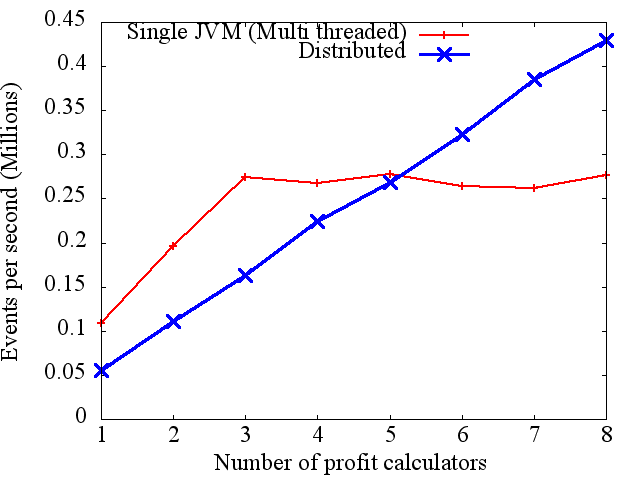
\includegraphics[width=3.0in]{throughput_profit.png}
        \caption{Throughput variation with the number of \textit{ProfitCalculator} instances.}
        \label{throughput_profit}
\end{figure}
 
Figure \ref{throughput_profit} shows the throughput variation for both setups. For single JVM set up initially throughput increases, due to increment of parallelism and comes to a steady state. For distributed setup  throughput increases linearly, although it has an initial lesser throughput compared to single JVM setup due to message serialization, message deserialization and TCP overheads. 

\begin{figure}[!t]
        \centering
        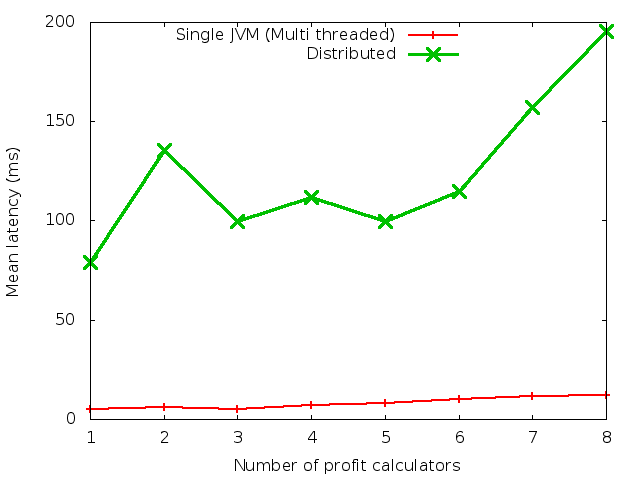
\includegraphics[width=3.0in]{latency_profit.png}
        \caption{Mean latency variation with the number of \textit{ProfitCalculator} instances.}
        \label{latency_profit}
\end{figure}

Figure \ref{latency_profit} shows the latency variation for both setups. For single JVM, latencies slightly increased with the addition of new instances as expected. But for distributed setups latency linearly increases with the addition of new nodes after 6 \textit{ProfitCalculator} instances. This latency increment is due to longer queues at the \textit{TopProfitProcessor}. In our message ordering process, we can send a message to \textit{TopProfitProcessor} only if all queues are not empty. This allows some processes with less top ten profitable events to delay other process messages. This problem can  possibly fixed by adding a limit to the message queue size. On the other hand in a real time system, this event ordering many not required since event processing happens at real time.

\subsection{Scalability with Window Size}

The grand challenge problem uses 15 minute window size for profitable cells query. However in a real world problems window sizes may required. Therefore finally we evaluated scalability of our solution with the window size.  For this experiment, we measured the throughput of the profitable cells query using a single JVM and three instances by varying the window size. Further we compared the throughput with our \textit{DynamicHeap} based solution which is not effective in lower window sizes as well.

\begin{figure}[!t]
        \centering
        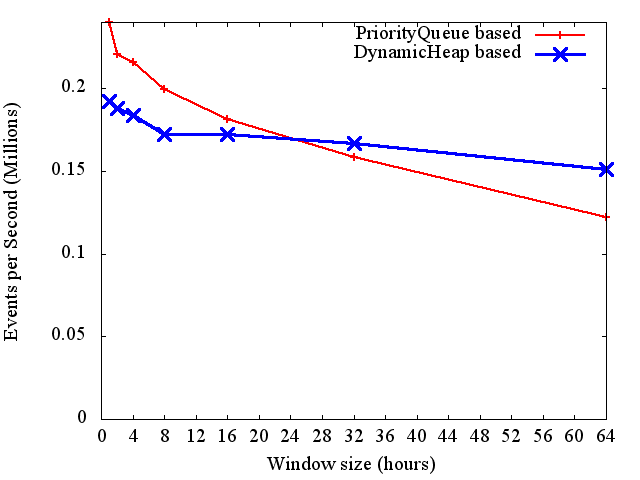
\includegraphics[width=3.0in]{window.png}
        \caption{Throughput variation with the window size.}
        \label{window}
\end{figure}

Figure \ref{window} shows the results. For both solutions, throughput does not drop by half, even though the window size increases 64 times. And for large windows \textit{DynamicHeap} performs better than the \textit{PriorityQueue} based one. This is due to two reasons. Firstly, all operations of \textit{DynamicHeap} are O(log(n)). Secondly, out of 173 million records there are only around 18000 unique fares. Therefore \textit{DyamicHeap} based algorithm does not consume memory beyond that. However , since \textit{PriortyQueue} based implementation keeps all values in memory it consumes more memory for large windows.


%
% The following two commands are all you need in the
% initial runs of your .tex file to
% produce the bibliography for the citations in your paper.
\bibliographystyle{abbrv}
\bibliography{sigproc}  % sigproc.bib is the name of the Bibliography in this case
% You must have a proper ".bib" file
%  and remember to run:
% latex bibtex latex latex
% to resolve all references
%
% ACM needs 'a single self-contained file'!
%
%APPENDICES are optional
%\balancecolumns
%Appendix A
% That's all folks!
\end{document}
